\section{Results}
\label{sec:results}

The results first show how the PTES is used under the existing monthly tariff, then how the derived credit changes HTF's response in individual weeks, and finally the effect over the year and its distribution between HTF and the upstream side. Unless stated otherwise, the hourly credit refers to Eq.~\eqref{eq:bounded-credit} with $g=0.25$ and a mean of 5~DKK/MWh.

\subsection{PTES use under the monthly tariff}
\label{sec:results-reference}

The measured 2024 operation corresponds to approximately 10 equivalent full cycles, below the intended range of 25--30 cycles per year \cite{sifnaios2025performance}. Figure~\ref{fig:ptes_real_soc} shows the observed state of charge. The recorded charging and discharging volumes are derived from changes in the state of charge and are therefore used as context, not as a calibration target.

\begin{figure}[!htb]
    \centering
    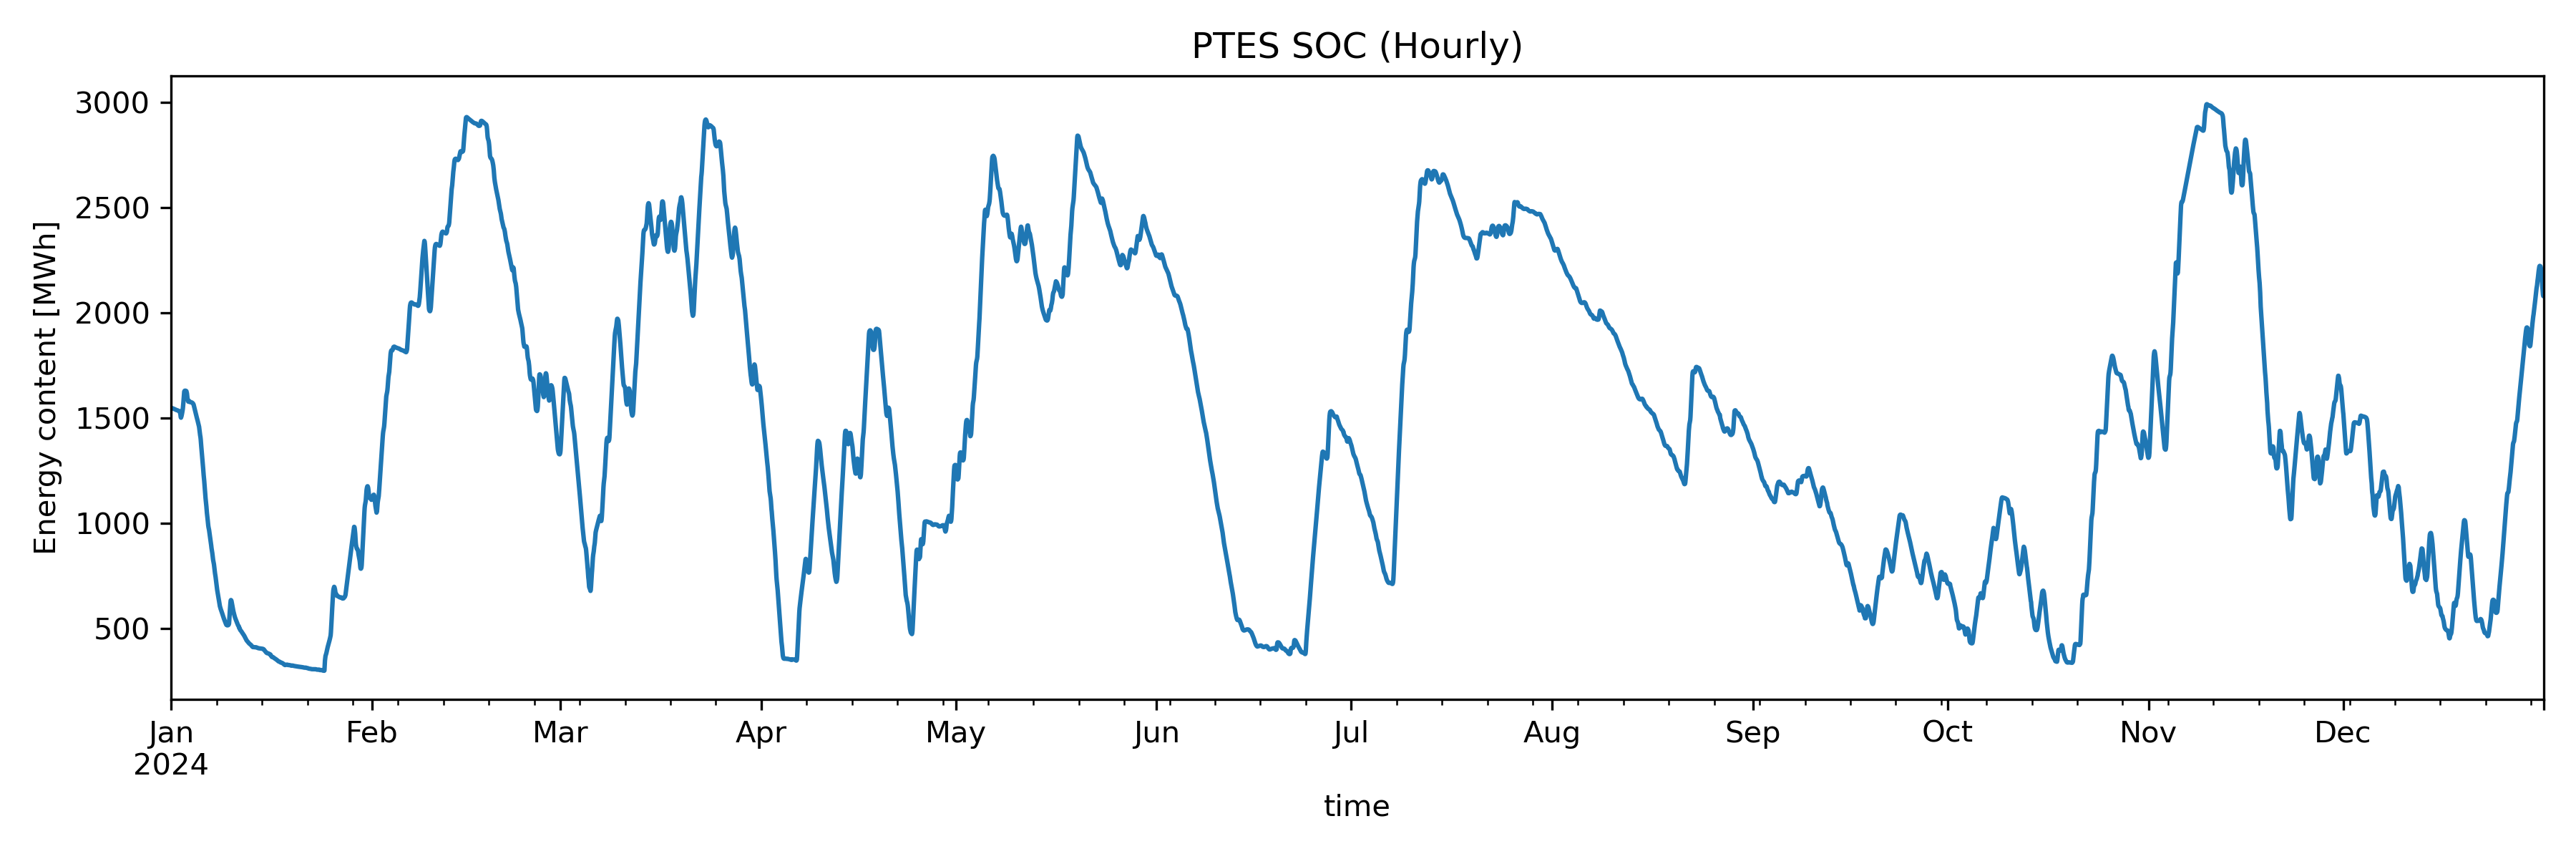
\includegraphics[width=0.9\linewidth]{figures/paper_figure/ptes_soc_hourly.png}
    \caption{Observed state of charge of the PTES in 2024, derived from measured operational data.}
    \label{fig:ptes_real_soc}
\end{figure}

In the model, the coordinated schedule uses the PTES for 21.6 equivalent full cycles over the 52 weeks of 2024 (71.3~GWh discharged). When HTF responds to the monthly tariff, discharge falls to 0.5~GWh, or 0.14 cycles, and occurs in only six weeks. The PTES is charged only to compensate standing losses. This is the incentive mismatch of Section~\ref{sec:case_study}: discharged heat costs HTF the same as direct heat but adds pumping electricity, so a cost-minimising HTF imports directly. The observed ten cycles lie between these two benchmarks, which is consistent with a storage that is scheduled centrally but implemented by an operator without a financial reason to follow the schedule.

The difference between the reference response and the coordinated schedule is the coordination value of the PTES. It amounts to 4.8~MDKK over the year. It varies strongly between weeks, from 7~kDKK in early January to more than 300~kDKK in individual weeks in September and December (Figure~\ref{fig:annual-weeks}a).

\subsection{Tariff signal and HTF response in individual weeks}
\label{sec:results-weeks}

Figure~\ref{fig:week-detail} shows a shoulder week in April and a summer week in July. The marginal values of delivered heat and of stored heat (panel a) are nearly constant within each week, although electricity prices vary strongly. The two large accumulators already smooth the upstream heat cost over the day, so the PTES adds value mainly by shifting heat over several days. In the summer week both values are negative: additional heat demand allows the back-pressure CHP units to produce more electricity at high prices, which reduces net system cost.

\begin{figure}[!htb]
    \centering
    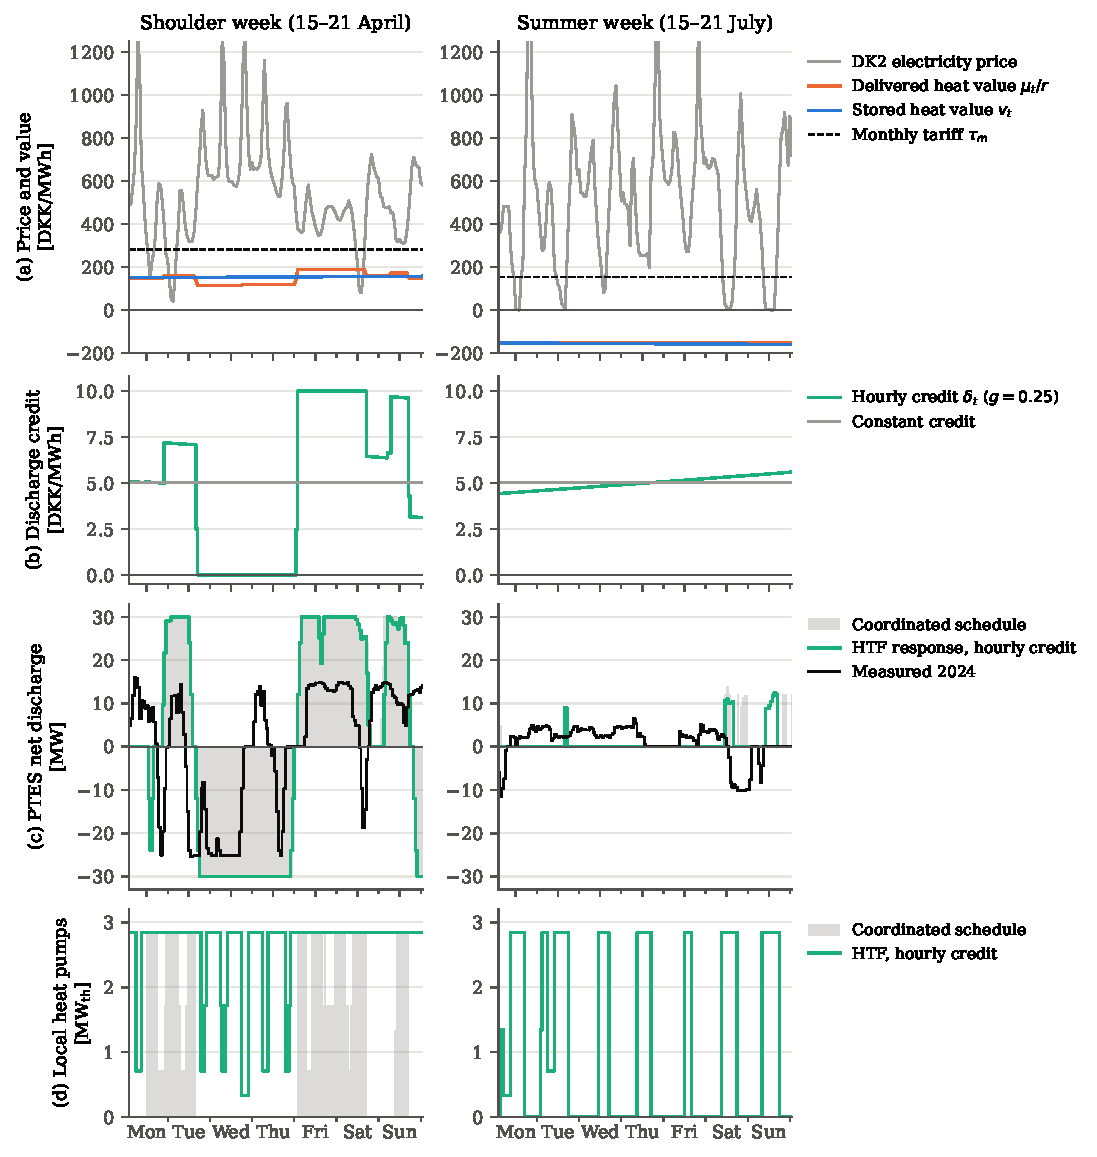
\includegraphics[width=\linewidth]{figures/04_Results/week_detail.pdf}
    \caption{Shoulder (left) and summer (right) week of 2024. (a) DK2 electricity price, conditional values of delivered and stored heat, and the monthly tariff. (b) Hourly discharge credit and the constant credit with the same mean. (c) PTES net discharge (positive) and charging (negative). (d) Output of the two local heat pumps.}
    \label{fig:week-detail}
\end{figure}

The credit (panel b) follows the spread between the two values. In the shoulder week it is zero on Wednesday and Thursday, when stored heat is worth more than delivered heat and the PTES is charged, and reaches the 10~DKK/MWh bound on Friday and Saturday, when the coordinated schedule discharges. With either credit, HTF's discharge follows the coordinated schedule closely (panel c), because any credit above the pumping cost, about 3~DKK/MWh on average, makes discharge attractive. The hourly credit additionally removes discharge in hours where it is not useful. With the constant credit, HTF discharges in single hours outside the scheduled blocks, for example at the start of the shoulder week and in the second half of the summer week. In these hours the system would rather keep the heat for later.

Panel (d) shows that HTF's heat pumps run much more than in the coordinated schedule. In the summer week the coordinated schedule does not use them at all, because the system value of heat is negative, while HTF compares them with a monthly tariff of 153~DKK/MWh. The discharge credit does not change this decision.

\subsection{Annual effect and distribution between stakeholders}
\label{sec:results-annual}

Figure~\ref{fig:annual-weeks} and Table~\ref{tab:annual-results} summarise the 52 weeks. With the hourly credit, PTES discharge rises to 68.5~GWh, or 20.8 cycles, which is 96\% of the coordinated schedule. The system operating saving relative to the monthly tariff is 3.92~MDKK, or 81\% of the coordination value. The constant credit with the same mean gives 3.54~MDKK. The difference of 0.38~MDKK is the value of timing alone, since both credits have the same average level.

\begin{figure}[!htb]
    \centering
    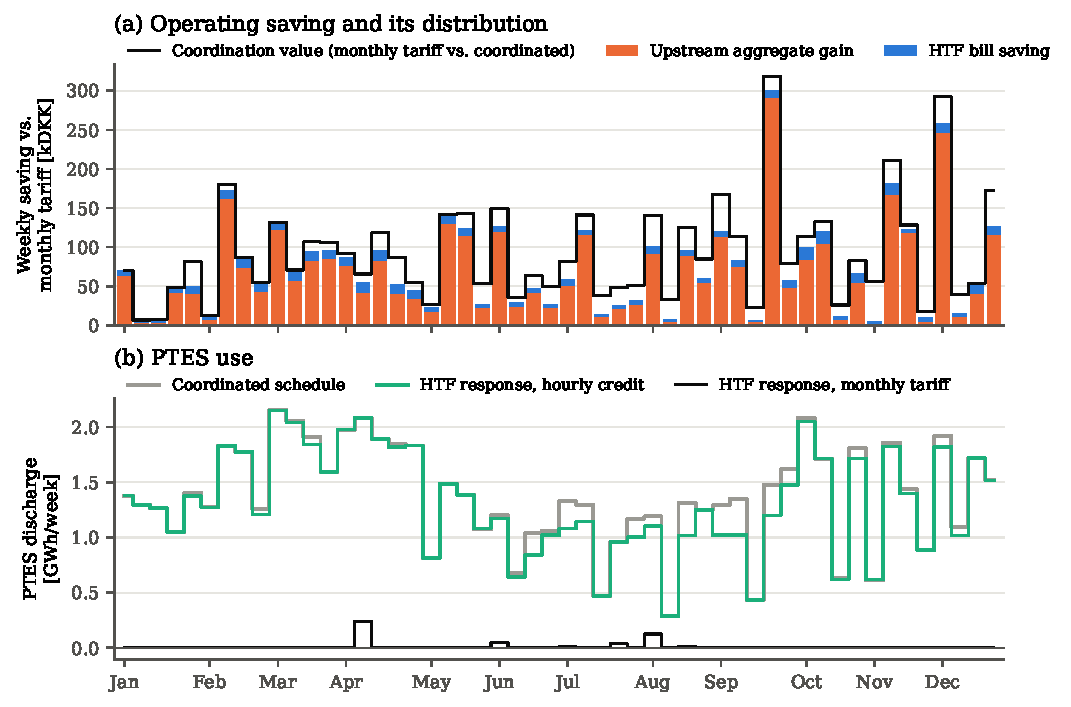
\includegraphics[width=\linewidth]{figures/04_Results/annual_weeks.pdf}
    \caption{Weekly results for 2024 under the hourly discharge credit. (a) Operating saving relative to the monthly tariff, split into HTF's bill saving and the upstream aggregate gain, and the coordination value of each week. (b) Weekly PTES discharge in the coordinated schedule and in HTF's response to the monthly tariff and to the hourly credit.}
    \label{fig:annual-weeks}
\end{figure}

\begin{table}[!htb]
    \centering
    \small
    \caption{Annual results, summed over the 52 weekly benchmarks of 2024, relative to HTF's response to the monthly tariff. Savings in MDKK; positive values are gains.}
    \label{tab:annual-results}
    \begin{tabular}{lrrr}
        \toprule
        & Constant credit & Hourly credit & Hourly credit and \\
        & 5 DKK/MWh & $g=0.25$ & hourly direct heat \\
        \midrule
        System operating saving $\Delta C^{\mathrm{sys}}$ & 3.54 & 3.92 & 3.95 \\
        HTF bill saving $\Delta B^{\mathrm{HTF}}$ & 0.20 & 0.40 & 0.49 \\
        Upstream aggregate gain $\Delta U$ & 3.34 & 3.52 & 3.46 \\
        \quad of which change in heat revenue & $-0.34$ & $-0.55$ & $-0.55$ \\
        Recovered coordination value $\rho$ & 73\% & 81\% & 82\% \\
        PTES discharge [GWh] & 67.5 & 68.5 & 68.3 \\
        Equivalent full cycles & 20.4 & 20.8 & 20.7 \\
        Weeks in which both sides gain & 51 & 52 & 46 \\
        \bottomrule
    \end{tabular}
\end{table}

Both sides gain from the hourly credit. HTF saves 0.40~MDKK, about 5.8~DKK per discharged MWh after paying the additional pumping electricity. The upstream side loses 0.55~MDKK of heat revenue because discharged heat is billed at a lower price, but its operating cost falls by more, so its aggregate gain is 3.52~MDKK. The gain holds in every week (Figure~\ref{fig:annual-weeks}a): no week requires a transfer to keep either side whole. HTF receives about 10\% of the value created, measured as 57~DKK per discharged MWh. The constant credit benefits both sides in 51 of the 52 weeks; in the remaining winter week, the upstream side loses 64~DKK because untimely discharge raises standing losses.

\subsection{Heat pumps: what a discharge tariff cannot fix}
\label{sec:results-hp}

The hourly credit leaves 0.9~MDKK, or 19\% of the coordination value, unrecovered. This remainder is not caused by the PTES, whose discharge follows the coordinated schedule closely. It is caused mainly by HTF's heat pumps. Over the year they produce 17.0~GWh in HTF's response but only 9.9~GWh in the coordinated schedule. The difference arises from March to November, when the system value of delivered heat averages between $-22$ and 149~DKK/MWh while the monthly tariff averages between 165 and 262~DKK/MWh. HTF then saves money by producing heat locally, although the system has cheaper heat available.

Making the direct-heat price hourly while keeping its monthly mean recovers only 0.03~MDKK more and reduces HTF's heat-pump output by just 0.4~GWh. The cause is the price level, not its timing: the monthly tariff lies well above the marginal value of heat for most of the year, so a signal that preserves its mean still makes local heat pumps attractive. The hourly direct price also shifts costs to HTF in several winter and late-autumn weeks, which leaves HTF worse off in 6 of the 52 weeks. Aligning heat-pump operation would therefore require a separate signal for local production, for example a heat-pump-specific price or a two-part tariff, rather than a change in the timing of the existing tariff.
